\section{Events, Probability and Random Variables}
The course aims to develop an abstract mathematical framework to describe the likelihood of certain events to happen in a random experiment. We would like to also formalise the large-sample results as developed in the probability classes you have taken in lower years, including the \textit{Law of Large Numbers} and \textit{Central Limit Theorem}.\\

To begin the story, we should understand how one can describe an experiment. You should have seen in previous probability courses that there are few key steps \footnote{as suggested in Dr. Chris Hallsworth notes on MATH50010 Probability for Statistics.} to describe an experiment:
\begin{enumerate}
    \item First describe the sets of possible outcomes $\omega$ of the experiment, which is known as \textit{sample space} $\Omega$. 
    \item Then describe the \textit{events} $A$ which we might observe as subsets of the sample space $\Omega$. We usually write the collection of such subset as $\F$. 
    \item Finally, assign a number $\p(A) \in [0,1]$ (included) to each of the subsets $A$ to quantify how likely this event might happen.
\end{enumerate}

This leads to the following fundamental problem:
\begin{itemize}
    \item What should we include in our collection of events $\F$, and
    \item How should we assign a number to those subsets in $\F$?
\end{itemize}

Let us first address the first question. For the description to make sense in reality, we should let $\F_* := \set{\varnothing, \Omega} \subseteq \F$, since we should definitely observe nothing or something in an experiment. In fact, we should probably including more subsets of $\Omega$ in $\F$ for our description to be useful. \\

A natural choice is to choose $\F = \F^* := 2^\Omega$, the \textit{power set} of $\Omega$ (which contains all subsets of $\Omega$). This is fine if $\Omega$ is countable, but will raise some issue if $\Omega$ is uncountable, e.g. $\Omega = \R$. The main concern comes from our second question: there are many properties we wish $\p$ to satisfy, e.g.  finite additivity: 

$$\forall A,B \in \F \text{ disjoint, } \p(A\cup B) = \p(A) + \p(B)$$

We can extend this naturally to countable additivity, and you should have seen that those properties would lead to contradictions! \footnote{e.g. Vitali sets, Banach-Tarski paradox. See MATH50006 Lebesgue Measure and Integration.} Therefore, we should choose $\F$ that contains $\F_*$ but is strictly smaller than $2^\Omega$.\\

Mathematicians had therefore attempted to find suitable criteria on $\F$ and $\p$ so that they would not give rise to contradictions, but still allow $\F$ to be large enough for our framework to be useful. The most successful attempt was, perhaps, made by Andrey Kolmogorov in 1933 when he devised the axioms of probability in his \textit{Grundbegriffe der Wahrscheinlichkeitsrechnung} (Foundations of the Theory of Probability), which we will cover in this chapter. His work lead to the development of the \textit{measure theory}, which forms the fundamentals of our probability theory.\\

As a final remark, the first two chapters of this course have many overlap with the courses you have done in year 1-2, so if you are familiar with the notions in these chapters, you can safely skip ahead.
\newpage

\subsection{Algebras and $\sigma$-algebras}
Let $\Omega$ be a set of points $\omega$. 
\begin{definition}[Algebra and $\sigma$-algebra] A nonempty system of subsets of $\Omega$ is called an \textbf{algebra} $\A$ if 
    \begin{itemize}
        \item $\Omega \in \A$
        \item $A,B \in \A \implies A \cup B \in A \quad (A \cap B \in \A)$
        \item $A \in \A \implies A^c \in \A$
    \end{itemize}
In addition, if all countable union $\bigcup_{n=1}^\infty A_n \in \A$ whenever $A_1, A_2, \dots \in \A$, then $\A$ is a $\sigma$-algebra. Note that then also $\bigcap_{n=1}^\infty A_n \in \F$ (consider $\Omega \backslash A_k = \hat{A}_k$).
\end{definition}

\begin{definition}[Set function and measures]
    \begin{itemize}
    \item[]
    \item A set function $\mu : \A \longrightarrow [0, \infty]$ is \textbf{finitely additive} if for any disjoint $A,B \in \A$
    \begin{equation*}
        \mu(A\cup B) = \mu(A) + \mu(B).
    \end{equation*}
    Note that then $\forall A,B \in \A$
    \begin{equation*}
        \mu(A \cup B) = \mu(A)+\mu(B) - \mu(A \cap B).
    \end{equation*}
    \item Let $\F$ be a $\sigma$-algebra. A set function $\mu : \F \rightarrow [0, \infty]$ is called $\bm{\sigma}$\textbf{-additive} if for any disjoint $A_1, A_2, ... \in \F$,
    \begin{equation*}
        \mu \bigg(\bigcup_{n=1}^\infty A_n\bigg) = \sum_{n=1}^\infty \mu(A_n). 
    \end{equation*}
    Such $\mu$ is called a \textbf{measure} on $\F$. A measure $\mu$ is called a \textbf{probability measure} if $\mu (\Omega) = 1$. Note that $\mu (\varnothing) = 0$ since $\mu(\varnothing) = \mu (\varnothing\cup \varnothing) = 2\mu (\varnothing)$. 
    \item A measure is called $\bm{\sigma}$\textbf{-finite} if there exists a representation $\Omega = \bigcup_{k=1}^\infty \Omega_k$, $\Omega_k$ - pairwise disjoint, with
    \begin{equation*}
        \mu(\Omega_k)<\infty, \quad k = 1,2,...
    \end{equation*}
\end{itemize}
\end{definition}

\begin{definition}
A \textbf{probability space} is a triple $(\Omega ,\F, \p)$, where $\Omega$ is a set called sample space, $\F$ is a $\sigma$-algebra of subsets of $\Omega$, $\p$ is a probability measure on $\F$. Any element of $\F$ is called an \textbf{event}.
\end{definition}
\begin{property}
Probability measures have the following properties:
\begin{itemize}
    \item $\p(\varnothing) = 0$;
    \item If $A,B \in \F$ then
    \begin{equation*}
        \p(A\cup B) = \p(A) + \p(B) - \p(A\cap B);
    \end{equation*}
    \item If $A,B \in \F$ and $B\subseteq A$ then
    \begin{equation*}
        \p(B) \le \p(A);
    \end{equation*}
    \item If $A_1, A_2, \dots \in \F$, then 
    \begin{equation*}
        \p \bigg( \bigcup_{n=1}^\infty A_n \bigg) \le \sum_{n=1}^\infty \p (A_n).
    \end{equation*}
\end{itemize}
\end{property}

\begin{proposition}
Let $\p$ be a finitely additive set function defined over an algebra $\A$, with $\p(\Omega) = 1$. The following four conditions are equivalent:
\begin{enumerate}[(1)]
    \item $\p$ is $\sigma$-additive (therefore it is a probability)
    \item $\p$ is continuous from below, i.e. for any sets $A_1, A_2, \dots \in \A$ such that $A_1 \subset A_2 \subset \dots$ and $\bigcup_{n=1}^\infty A_n \in \A$,
    \begin{equation*}
        \p \bigg( \bigcup_{n=1}^\infty A_n \bigg) = \lim_{n \rightarrow \infty} \p (A_n);
    \end{equation*}
    \item $\p$ is continuous from above, i.e. for any sets $B_1, B_2, \dots$ such that $B_1 \supset B_2 \supset \dots$ and $\bigcap_{n=1}^\infty B_n \in \A$,
    \begin{equation*}
        \lim_{n\rightarrow \infty} \p(B_n) = \p \bigg( \bigcap_{n=1}^\infty B_n\bigg);
    \end{equation*}
    \item $\p$ is continuous at $\varnothing$, i.e. for any sets $B_1, B_2, \dots \in \A$ such that $B_1 \supset B_2 \supset \dots$ and $\bigcap_{n=1}^\infty B_n =\varnothing$,
    \begin{equation*}
        \lim_{n \rightarrow \infty} \p(B_n) = 0.
    \end{equation*}
\end{enumerate}
\end{proposition}

\begin{proof}
$(1) \implies (2)$. Since
\begin{equation*}
    \bigcup_{n=1}^\infty A_n = A_1 + (A_2\backslash A_1) + (A_3\backslash A_2) + \cdots,
\end{equation*}
we have
\begin{align*}
    \p \bigg( \bigcup_{n=1}^\infty A_n \bigg) &= \p(A_1) + \p(A_1\backslash A_2) + \p(A_3\backslash A_2) + \cdots\\
    &= \p(A_1) + \p(A_2) - \p(A_1) + \p(A_3) - \p(A_2) + \cdots\\
    &= \lim_{n\rightarrow \infty} \p(A_n).
\end{align*}
$(2) \implies (3)$. Let $n \ge 1$; then
\begin{equation*}
    \p(B_n) = \p(B_1 \backslash (B_1 \backslash B_n)) = \p (B_1) - \p(B_1 \backslash B_n).
\end{equation*}
The sequence $\{ B_1 \backslash B_n \}_{n\ge1}$ of sets is non-decreasing and 
\begin{equation*}
    \bigcup_{n=1}^\infty (B_1 \backslash B_n) = B_1 \backslash \bigcap_{n=1}^\infty B_n.
\end{equation*}
Then by $(2)$
\begin{equation*}
    \lim_{n \rightarrow \infty} \p(B_1 \backslash B_n) = \p \bigg( \bigcup_{n=1}^\infty (B_1 \backslash B_n)\bigg)
\end{equation*}
and therefore
\begin{align*}
    \lim_{n \rightarrow \infty} \p(B_n) &= \p(B_1) - \lim_{n \rightarrow \infty} \p(B_1 \backslash B_n)\\
    &= \p(B_n) - \p \bigg( \bigcup_{n=1}^\infty (B_1 \backslash B_n)\bigg) = \p(B_1) - \p \bigg( (B_1 \backslash \bigcap_{n=1}^\infty B_n)\bigg)\\
    &= \p (B_1) - \p (B_1) + \p \bigg( \bigcap_{n=1}^\infty  B_n\bigg) = \p \bigg( \bigcap_{n=1}^\infty  B_n\bigg).
\end{align*}
$(3) \implies (4)$. Obvious.

$(4) \implies (1)$. Let $A_1, A_2, \dots \in \A$ be pairwise disjoint and let $ \sum_{n=1}^\infty A_n \in \A$. Then 
\begin{equation*}
    \p \bigg( \sum_{i=1}^\infty A_i \bigg) = \p \bigg( \sum_{i=1}^n A_i\bigg) + \p \bigg( \sum_{i=n+1}^\infty A_i \bigg),
\end{equation*}
and since $\sum_{i=n+1}^\infty A_i \downarrow \varnothing, n\rightarrow \infty$, we have 
\begin{align*}
    \sum_{i=1}^\infty \p(A_i) &= \lim_{n \rightarrow \infty} \sum_{i=1}^n \p(A_i) = \lim_{n \rightarrow \infty} \p \bigg( \sum_{i=1}^n A_i\bigg)\\
    &= \lim_{n \rightarrow \infty} \bigg[ \p\bigg( \sum_{i=1}^\infty A_i\bigg) - \p\bigg( \sum_{i=n+1}^\infty A_i\bigg) \bigg]\\
    &= \p \bigg( \sum_{i=1}^\infty A_i \bigg) - \lim_{n \rightarrow \infty}  \p \bigg( \sum_{i=n+1}^\infty A_i \bigg) =  \p \bigg( \sum_{i=1}^\infty A_i \bigg).
\end{align*}
\end{proof}



\begin{proposition}
Let $\mu$ be a finitely additive measure on an algebra $\A$ and let the sets $A_1, A_2, \dots \in \A$ be pairwise disjoint and satisfy $A = \bigcup_{i=1}^\infty A_i \in \A$. Then 
\begin{equation*}
    \sum_{i=1}^\infty \mu (A_i) \le \mu(A).
\end{equation*}
\end{proposition}

\begin{example}[$\sigma$-algebras on $\Omega$] 
Let $\Omega$ be a sample space. The following are $\sigma$-algebras:
\begin{equation*}
    \F_* = \{ \varnothing, \Omega \}; \quad \F^* = \{ A: A \in \Omega \} = 2^\Omega;
\end{equation*}
\end{example}

\begin{lemma}
For any collection $\mathcal{E}$ of subsets of $\Omega$ there exists minimal algebra $a (\mathcal{E})$ and minimal $\sigma$-algebra $\sigma(\mathcal{E})$ that contains all elements of $\mathcal{E}$ (intersection of all algebras (resp. $\sigma$-algebras) containing $\mathcal{E}$).
\end{lemma}
\begin{proof}
Intersection, countable or uncountable, of algebras (resp. $\sigma$-algebras) containing $\mathcal{E}$ is an algebra (resp. $\sigma$-algebra) containing $\mathcal{E}$.
\end{proof}
We say that $\sigma (\mathcal{E})$ is \textbf{generated} by $\mathcal{E}$.

\begin{example}[$\sigma$-algebra generated by partitions] Let $D = \{ D_1, D_2, \dots \}$ be a countable partition of $\Omega$ such that $\Omega = \bigsqcup_{j=1}^\infty D_j$. Then
\begin{equation*}
    \sigma(D) = \bigg\{ \bigcup_{j \in I}D_j : I \subset \mathbb{N} \bigg\},
\end{equation*}
To show this, we first note that the RHS is indeed a $\sigma$-algebra containing $D$. (Exercise!) Therefore we must have $\sigma(D) \subseteq$ the RHS. But since $\sigma(D)$ is closed under countable union we know that the RHS must be a subset of $\sigma(D)$. This proves the claim.
\end{example}

\subsection{Measurable Spaces}
\begin{definition}
A \textbf{measurable space} is a pair $(E, \mathcal{E})$, where $E$ is a set and $\mathcal{E}$ is a $\sigma$-algebra on $E$.
\end{definition}
\subsubsection{The measurable space $(\R, \B(\R))$}
Let $\R = (-\infty, \infty)$ be the real line and
\begin{equation*}
    (a,b] = \{ x \in \R : a < x \le b \},
\end{equation*}
for all $a,b$ with $-\infty \le a < b < \infty$. Let $\A$ be the algebra of subsets of $\R$ such that
\begin{equation*}
    A \in \A \quad \text{if} \quad  A = \bigcup_{i=1}^n (a_i, b_i] \quad n <\infty.
\end{equation*}
Let $\B(\R)$ be the smallest $\sigma$-algebra $\sigma(\A)$ containing $\A$. We observe that 
\begin{align*}
    (a,b) &= \bigcup_{n=1}^\infty \bigg(a,b-\frac{1}{n} \bigg], \quad a<b,\\
    [a,b] &= \bigcap_{n=1}^\infty \bigg(a - \frac{1}{n},b\bigg], \quad a<b,\\
    \{a\} &= \bigcap_{n=1}^\infty \bigg(a - \frac{1}{n},a\bigg].
\end{align*}
Thus the Borel algebra contains not only intervals $(a,b]$ but also the singletons $\{ a\}$ and all sets of the forms 
\begin{equation*}
    (a,b), \quad [a,b], \quad [a,b), \quad (-\infty,b), \quad (-\infty,b], \quad (a,\infty).
\end{equation*}
Let us also notice that the construction of $\B(\R)$ could have been based on any of the intervals above instead of on $(a, b]$, since all the minimal $\sigma$-algebras generated by systems of intervals of any of the forms are the same as $\B(\R)$.

\begin{exercise}
Show that $\B(\R)$ is generated by the collection of (1) open intervals of the form $(a,b)$, (2) closed intervals $[a,b]$, (3) half intervals, (4) intervals of the form $(-\infty, a]$ or $[a,\infty)$, (5) open sets and (6) closed sets with respect to the Euclidean metric.
\end{exercise}

\subsubsection{The measurable space $(\mathbb{R}^n, \B(\mathbb{R}^n))$}
Let $\R^n = \R \times \cdots \R$ be the direct product of $n$ copies of the real line, i.e. the set of ordered $n$-tuples $x = (x_1,\dots,x_n)$, where $x_k \in \R, k = 1,\dots, n$. The set
\begin{equation*}
    I = I_1 \times \cdots I_n,
\end{equation*}
where $I_k = (a_k,b_k]$, i.e. the set $\{x\in \R^n: x_k \in I_k, k=1,...,n \}$ is called a rectangle and $I_k$ is a side of the rectangle. Let $\mathcal{I}$ be the set of all rectangles $I$. The smallest $\sigma$-algebra $\sigma(\mathcal{I})$ generated by the system $\mathcal{I}$ is the Borel algebra of subsets of $\R^n$. Let us show that we can arrive at this Borel algebra by starting in a different way.
\newline

Instead of the rectangles $I = I_1 \times \cdots I_n$ let us consider the rectangles $B = B_1 \times B_2 \times \cdots \times B_n$ with Borel sides ($B_k$ is the Borel subset of the real line that appears in the $k$th place in the direct product $\R \times \cdots \times \R$).The smallest $\sigma$-algebra containing all rectangles with Borel sides is denoted by
\begin{equation*}
    \B(\R) \otimes \cdots \otimes \B(\R)
\end{equation*}
and called the direct product of the $\sigma$-algebras $\B(\R)$. Let us show that in fact
\begin{equation*}
    \B(\R^n) = \B(\R) \otimes \cdots \otimes \B(\R).
\end{equation*}
In other words, the smallest $\sigma$-algebra generated by the rectangles $I = I_1 \times \cdots \times I_n$ and the (broader) class of rectangles $B = B_1 \times \cdots \times B_n$ with Borel sides are actually the same. We need the following lemma
\begin{lemma}
Let $\mathcal{E}$ be a class of subsets of $\Omega$ and let $\B \subseteq \Omega$, and define
\begin{equation*}
    \mathcal{E} \cap B = \{ A \cap B: A \in \mathcal{E}\}.
\end{equation*}
Then 
\begin{equation*}
    \sigma(\mathcal{E}\cap B) = \sigma(\mathcal{E})\cap B.
\end{equation*}
\end{lemma}
Now we show that $\B(\R^n)$ and $\B(\R) \otimes \cdots \otimes \B(\R)$ are the same. This is obvious for $n=1$. We now show that it is true for $n=2$.
\begin{lemma}
\begin{equation*}
    \B(\R^2) = \B(\R) \otimes \B(\R)
\end{equation*}
\end{lemma}
\begin{proof}
\begin{itemize}
    \item[]
    \item $\B(\R^2) \subset \B(\R) \otimes \B(\R)$, since any open $A \subset \bigcup_{x \in A\cap \mathbb{Q}^2} R(x, \sigma(x)) \in \B(\R) \otimes \B(\R)$, $R(x, \tau)$ - open square centered at $x$ of side length $\tau(x)$.
    \item $\B(\R) \otimes \B(\R) \subset \B(\R^2)$. It is sufficient to check that $B_1 \times B_2 \in \B(\R^2)$ for any $2$ Borel sets $B_1, B_2$. Note that $B_1 \times \R \in \B(\R^2)$ since 
    \begin{equation*}
        B_1 \times \R \in \sigma(\{ \text{open subsets of } \R \}) \times \R = \sigma (\{ \text{open subsets of }\R \times \R \}),
    \end{equation*}
    Similarly, $\R \times B_2 \in \B(\R^2)$, and so 
    $B_1 \times B_2 = (B_1 \times \R) \cap (\R \times B_2) \in \B(\R^2)$.
\end{itemize}
\end{proof}
The case for any $n, n >2$ can be discussed in the same way.
\begin{remark}
Let $\B_0 (\R^n)$ be the smallest $\sigma-$ algebra generated by the open "balls"
\begin{equation*}
    S_\rho (x^0) = \{ x \in \R^n: \rho_n (x, x^0) < \rho \}, \quad x^0 \in \R^n, \rho > 0,
\end{equation*}
in the metric 
\begin{equation*}
    \rho_n (x,x^0) = \sum_{k=1}^n 2^{-k} \rho_1(x_k, x_k^0),
\end{equation*}
where $x = (x_1, \dots, x_n),$ $x^0 = (x_1^0, \dots, x_n^0).$ Then $\B_0(\R^n) = \B(\R^n)$ (exercise).
\end{remark}

\subsubsection{The measurable space $(\R^\infty, \B(\R^\infty))$}
This space plays a significant role in probability theory, since it is used as the basis for constructing probabilistic models of experiments with infinitely many steps. Let $\R^\infty = \{  x = (x_1, x_2, \dots ), x_k \in \R \}$.
\begin{definition}
A set $C \subset \R^\infty$ is called \textbf{cylindrical} if it is of the form $C = \{ x \in \R^\infty :(x_1, x_2, ..., x_n) \in \tilde{C}_n \}$ for some $n \ge 1$ and $\tilde{C}_n \in \B(\R^n)$.
\end{definition}
Cylindrical sets form an algebra (check!) which generates a $\sigma$-algebra called cylindrical $\sigma$-algebra, denoted $\B(\R^\infty)$. One can verify that
\begin{equation*}
    \B(\R^\infty) = \sigma(\{ A_1 \times A_2 \times \cdots \subset \R^\infty, A_k \in \B(\R) \}).
\end{equation*}
\begin{example}
For all $c \in \R$, let $A = \{ x \in \R^\infty : \limsup_n x_n = \inf_n \sup_{k>n} x_k > c \}$. We have $A \in \B(\R^\infty)$: indeed
\begin{equation*}
    A = \bigcap_{n=1}^\infty \bigcup_{k = n+1}^\infty \{ x \in \R^\infty: x_k > c \} = (x_k > c \quad i.o.).
\end{equation*}
For all $c$ let 
\begin{equation*}
    B = \{ x \in \R^\infty: \liminf_n x_n = \sup_n \inf_{k>n} x_k > c \}.
\end{equation*}
We have $B \in \B(\R^\infty)$: indeed
\begin{equation*}
    B = \bigcap_{n=1}^\infty \bigcup_{k = n+1}^\infty \{ x \in \R^\infty: x_k > c \} = (x_k > c \quad ev.).
\end{equation*}
For all $c$, $D = \{ x\in \R^\infty : \lim_{n \rightarrow \infty} x_n = c \} \in \B(\R^\infty)$ (exercise).
\end{example}
Recall: non-decreasing function $g(x)$ on $\R$ is continuous up to possibly countably many discontinuities of first kind: $f(x+0),$ $f(x-0)$ both exist, but $f(x+0)-f(x-0) = h_x>0$. Moreover, the derivative $g'(x)$ exists Lebesgue a.e.

\begin{unexaminable}
\begin{remark} \label{rmk:PolishSpace} We can generalise the notion of Borel $\sigma$-algebra to other sample spaces. Assume $\Omega$ is \textbf{Polish}, i.e. a metric space which is
\begin{itemize}
    \item \textbf{complete}: all Cauchy sequences $(\omega_k)_{k\geq 1}$ has a limit $\omega \in \Omega$, and 
    \item \textbf{separable}: there exists a countable subset $E :=  \set{\omega_k}_{k\geq 1}$ which is dense in $\Omega$, or $\bar{E} = \Omega$
\end{itemize}
then we can define the Borel $\sigma$-algebra of $\Omega$ $\B(\Omega)$ as the smallest $\sigma$-algebra containing all open subsets of $\Omega$. We can then talk about the Borel $\sigma$-algbera of e.g. the space of all continuous function of $[0,1]$, $\Omega = C^0([0,1])$, equipped with the supremum metric $d(f,g) = \sup_{[0,1]} |f-g|$.
\end{remark}

In fact, we will look at probability measures on Polish space quite often in Chapter 5 when we talk about weak convergence. If you are not comfortable with dealing with general Polish spaces, just treat them as $(\R,\B(\R))$ for the first reading. However, we will still try to incorporate discussions about measures on a general Polish space as they laid the foundation of stochastic processes. A few applications include:
\begin{itemize}
\item Continuous-time random walk (e.g. Brownian motion) - this could obviously be viewed as an indexed family of real-valued random variable $B_t(\omega), t \geq 0$, but one can also treat it as \textbf{one single} random variable $B(\omega) \in C^0[0,1].$
\item Empirical processes (i.e. "sample" cumulative distribution function) - this is usually treated as a random variable with an output of a distribution function (as defined below).
\end{itemize}

Therefore, we would encourage you to understand important results related to measures on a general Polish space before delving deep into the theory of stochastic processes.
\end{unexaminable}

\subsection{Probability Measures on Measurable Spaces}
\subsubsection{Probability Distributions}
We begin by the following observation.
\begin{exercise}
Let $(\R, \B(\R), \p)$ be a probability space and denote $F(x) := \p(-\infty, x]\quad x \in \R$. Show that:
\begin{itemize}
    \item $F(x)$ is non-decreasing,
    \item $\lim_{x\rightarrow -\infty} F(x) = 0$, $\lim_{x \rightarrow \infty} F(x) = 1$, and
    \item $F(x)$ is continuous on the right for all $x \in \R$.
\end{itemize}
\end{exercise}


\begin{definition}
Every function $F: \R \longrightarrow [0,1]$ satisfying the above three conditions is called a \textbf{distribution function} (on  the real line $\R$).
\end{definition}

Thus to every probability measure $\p$ on $(\R, \B(\R))$, there corresponds a distribution function. In fact, the opposite is also true and there exists one to one correspondence between distribution functions and probability measures:
\begin{theorem}
Let $F = F(x)$ be a distribution function on $\R$. Then there exists a unique probability measure $\p$ on $(\R, \B(\R))$ such that $$\p(a, b] = F(b) - F(a),$$
for all $a,b, -\infty \le a < b < \infty.$
\end{theorem}

This relies on the following fundamental result in measure theory.
\begin{theorem}[Caratheodory Theorem]
Let $\mu_0$ be a $\sigma$-additive (pre-)measure on $(\Omega, \A)$, where $\A$ is an algebra of subsets of $\Omega$. Then there exists a unique measure $\mu$ on $(\Omega, \sigma(\A))$, such that 
\begin{equation*}
    \mu (A) = \mu_0(A) \quad \forall A \in \A.
\end{equation*}
\end{theorem}

We make a few remarks on this theorem, the first one being the completeness of measure. Recall the following:
\begin{definition}[Complete measure]
A measure $\mu$ on a $\sigma$-algebra $\Sigma$ on $\Omega$ is called complete if any subset of a set of measure zero (null sets) is measurable, i.e. belongs to $\Sigma$.
\end{definition}

We introduce this notion of completeness to avoid any caveats in proving results relating to measures. Note that $(\R, \B(\R), \p)$ with $\p$ constructed from the Caratheodory theory above is not complete ($\exists$ subsets of a Borel set which are not Borel). Fortunately, one can enlarge the $\sigma$-algebra so that it includes all null sets: if a measure $\mu$ on $\Sigma$ is not complete, it can be completed by extending $\Sigma$ to 
\begin{equation*}
    \overline{\Sigma} = \sigma(\Sigma \cup \{ B \in \Omega : B \subset A \in \Sigma, \mu(A) = 0 \}),
\end{equation*}

and the definition of $\mu$ so that $\mu(B) = 0$ for any $B$ being a subset of a null set. This is a fundamental result that should be checked by yourself. The completion of the measure obtained from the Caratheodory theorem is called the \textit{Lebesgue-Stiltjes measure}. In particular, the distribution function $F(x) = x$ corresponds to the Lebesgue measure on $\R$.\\

The second remark concerns measure determining sets. Given two measures $\mu, \nu$ defined on a common measurable space $(\Omega,\F)$. How many sets do we need to check for us to show that $\mu = \nu$? The Caratheodory Theorem suggests that one may look at the algebra $\A$ such that $\F = \sigma(\A)$, but the following theorem suggests that one might look at a far smaller collection of subsets of $\Omega$: 

\begin{theorem}[Measure Determining Set] \label{thm:measure_determining}
Consider a measurable space $(\Omega,\F)$ with measures $\mu, \nu$, and let $\cC$ be a $\pi$-system containing $\Omega$ (in the sense that $A, B \in \cC$ implies $A \cap B \in \cC$). If $\mu(B) = \nu(B)$ for all $B \in \cC$, then $\mu = \nu$.
\end{theorem}

The key idea is to note that the collection $\set{B \in \F \,|\, \mu(B) = \nu(B)}$ is a Dynkin $\lambda$-system (which is non-empty, closed under complement and countable disjoint union). Since $\cC$ above is a sub-collection of this collection, we know from $\pi$-$\lambda$ theorem that $\sigma(\cC)$ is contained in this collection. Therefore if one can show that $\sigma(\cC) = \F$ then we have proven $\mu = \nu$. We will not go through the technical details here.

\begin{example} \label{eg:measures_determined_by_open_closed_sets}
As an application, any probability measure on $(\R,\B(\R))$ is determined by open, closed or half-open intervals. In other words, e.g. if $\mu, \nu$ are probability measures on $(\R,\B(\R))$ such that $\mu(O) = \nu(O)$ for all $O$ being open intervals, then $\mu = \nu$.
\end{example}

\begin{unexaminable}
\begin{example}
We can generalise this to the following: for probability measure defined on a Polish space $(X,\B(X))$, it is determined by open or closed sets in the above sense.
\end{example}
\end{unexaminable}

\subsubsection{Continuity of Measures on $(\R, \B(\R))$}

\textbf{Discrete/Atomic measures} are measures $\p$ for which the corresponding distributions $F = F(x)$ are piecewise constant, changing their values at the points $x_1, x_2, \dots$ ($\Delta F(x_i) >0$, where $\Delta F(x) = F(x) - F(x^-))$. 
\begin{center}
    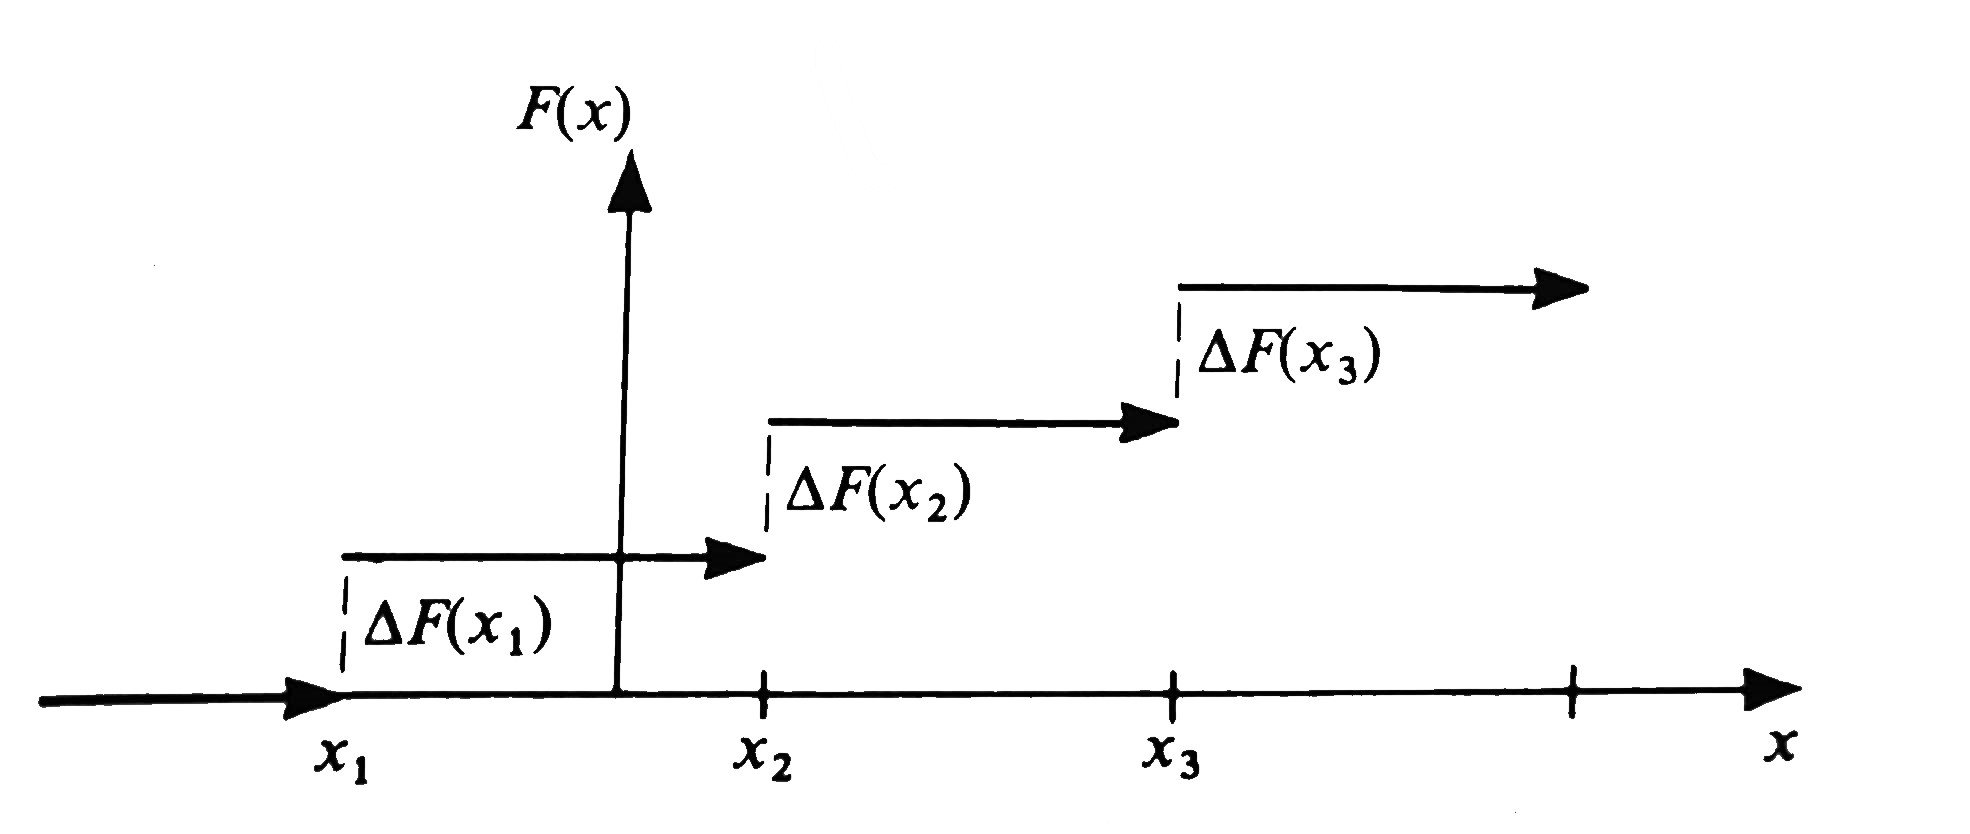
\includegraphics[scale = 0.2]{1.jpg}
\end{center}
In this case the measure is concentrated at the points $x_1, x_2, \dots$, known as \textbf{atoms}:
\begin{equation*}
    \p(\{ x_k \}) = \Delta F(x_k)>0, \quad \sum_k \p(\{x_k \}) = 1
\end{equation*}
The set of numbers $(p_1, p_2, \dots)$, where $p_k = \p\{x_k\}$, is called a \textbf{discrete probability distribution} and the corresponding distribution function 
\begin{equation*}
    F(x) = F_{\mathsf{disc}}(x) = \sum_{x_k \le x}p_k, \quad \quad \dots, p_1, p_2, \dots >0
\end{equation*}
is called \textbf{discrete}.
\begin{example}
\begin{itemize}
    \item[]
    \item Discrete Uniform distribution: $p_k = \frac{1}{N}, \quad k = 1,2,\dots, N, \quad N$ - fixed.
    \item Bernoulli $\sB(1,p)$: $p_1 = p, p_2 = 1-p,\quad 0 \le p \le 1.$
    \item Binomial $\sB(n,p)$: $p_k = \binom{n}{k} p^k (1-p)^k,\quad k = 0,1,\dots,n \quad 0 \le p \le 1.$
    \item Poisson $\Po(\lambda)$: $p_k = e^{-\lambda}\frac{\lambda^k}{k!}, \quad \lambda>0,\quad k = 0,1,\dots$
\end{itemize}
\end{example}
\textbf{Absolutely continuous measures}. We begin by noting the following observation:
\begin{proposition}
Let $f$ be an integrable function \footnote{see Chapter 2} $f(x) \ge 0$ such that
\begin{equation*}
    F(x) = F_{\mathsf{ac}}(x) = \int_{-\infty}^x f(t) \, \d t \quad \text{w.r.t Lebesgue measure}
\end{equation*}
Then the set function $\p_{ac}(A) = \int_{A} f(t)\d t \quad A \in \F$ is a measure. In particular, we say that $f$ is a density of $\p_{\mathsf{ac}}$.
\end{proposition}
\begin{proof}
First assign $\p_{ac}((a,b]) = \int_a^bf(t)\d t$, then use Caratheodory theorem to extend to $\sigma$-algebra.
\end{proof}
Measures of such kind is \textbf{absolutely continuous} (with respect to the Lebesgue measure $\mu$) in the following sense: if $\mu(A) = 0$ then $\p_{\mathsf{ac}}(A) = 0$. Indeed,

\begin{theorem}[Radon-Nikodym] If $\p$ is a measure such that $\mu(A) = 0\implies \p(A) = 0$, then $\p$ has a density.
\end{theorem}

Note that there is a connection between absolute continuity of measures and absolute continuity of measures: if $\p$ is an absolutely continuous measure then $F_{ac}(x)$ is an absolutely continuous function, and that $F'_{ac}(x) = f(x)$ almost everywhere.\\

Finally, the notion of absolute continuity can be generalised. This is useful in constructing conditional expectations: see Chapter 8.

\begin{example}
\begin{itemize}
    \item[]
    \item Uniform distribution on $[a,b]$: $f(x) = 1/(b-a), \quad a\le x \le b, \quad f(x) = 0$ otherwise.
    \item Normal or Gaussian: $f(x) = (2\pi \sigma^2)^{-1/2}\exp{\frac{-(x-m)^2}{2\sigma^2}}, \quad x \in \R, \quad \sigma >0.$
    \item Gamma: $f(x) = \frac{x^{\alpha - 1}e^{-x/\beta}}{\Gamma(\alpha)\beta^\alpha}, \quad x \ge 0 \quad \alpha, \beta >0$
\end{itemize}
\end{example}
Recall that a measure $\nu$ is said to be \textbf{concentrated} on a measurable set $A$ if $\nu(E) = 0$ for any $E \subset \R\backslash A$.\\

\textbf{Singular continuous}. These are measures whose distribution functions are continuous but have all their points of increases on sets of zero Lebesgue measure. We have that $F(x) = F_{\mathsf{sc}}(x)$ is continuous at any $x$ and $\p_{\mathsf{sc}}$ is concentrated on a set of Lebesgue measure zero. In particular this distribution has no atoms. For $x$ in this set, $F'_{\mathsf{sc}}(x) \ne 0$ or does not exist. Thus $F'_{sc}(x) = 0$ a.e. Note that, by continuity, $\p_{\mathsf{sc}}\{x\} = 0$ for each point $x\in \R$.
\begin{example}[Cantor's Devil staircase]
We consider the interval $[0,1]$ and construct $F(x)$ by the following procedure originated by Cantor. 
\begin{center}
    \begin{tikzpicture}
    \begin{axis}[
    axis lines=left,
    xlabel = $x$, ylabel = $F(x)$,
    xmax = 1.1, xtick = {0, 1/3, 2/3, 1}, 
    ymax = 1.1, ytick = {0, 1/2, 1},
    xticklabels={$0$, $1/3$, $2/3$, $1$},
    yticklabels={$0$, $1/2$, $1$}, 
    width=0.6\textwidth, height=0.4\textwidth]
    \addplot[domain=0:1/3] {3*x/2};
    \addplot[domain=1/3:2/3] {1/2};
    \addplot[domain=2/3:1] {3*(x-1)/2 + 1};
    \end{axis}
\end{tikzpicture}
\end{center}
We divide $[0,1]$ into thirds and put 
\begin{equation*}
    F_2(x) =
    \begin{cases}
     1/2, & x\in (\frac13, \frac23)\\
     1/4, & x \in (\frac19, \frac29)\\
     3/4, & x \in (\frac79, \frac89)\\
     0, & x = 0\\
     1, & x=1
    \end{cases}
\end{equation*}
defining it in the intermediate intervals by linear interpolation. Then we divide each of the intervals $[0,1/3]$ and $[2/3, 1]$ into three parts and define the function shown below with its values at other points determined by linear interpolation.
\begin{center}
    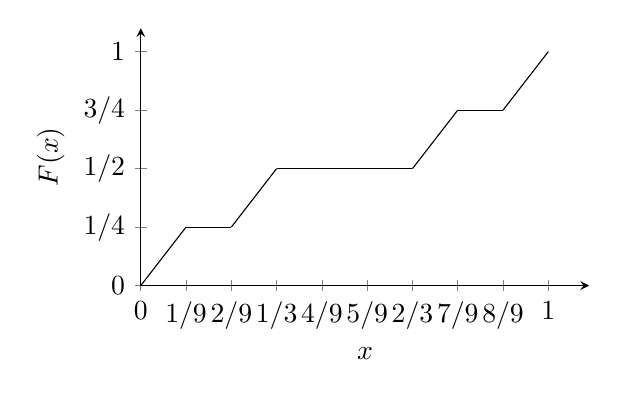
\begin{tikzpicture}
    \begin{axis}[
    axis lines=left,
    xlabel = $x$, ylabel = $F(x)$,
    xmax = 1.1, xtick = {0, 1/9, 2/9, 3/9, 4/9, 5/9, 6/9, 7/9, 8/9, 1}, 
    ymax = 1.1, ytick = {0, 1/4, 1/2, 3/4, 1},
    xticklabels={$0$, $1/9$, $2/9$, $1/3$, $4/9$, $5/9$, $2/3$, $7/9$, $8/9$, $1$},
    yticklabels={$0$, $1/4$, $1/2$, $3/4$, $1$}, 
    width=0.6\textwidth, height=0.4\textwidth]
    \addplot[domain=0:1/9] {9*x/4};
    \addplot[domain=1/9:2/9] {1/4};
    \addplot[domain=2/9:1/3] {9*(x-1/3)/4 + 1/2};
    \addplot[domain=1/3:2/3] {1/2};
    \addplot[domain=2/3:7/9] {9*(x-7/9)/4 + 3/4};
    \addplot[domain=7/9:8/9] {3/4};
    \addplot[domain=8/9:1] {9*(x-1)/4 + 1};
    \end{axis}
\end{tikzpicture}
\end{center}
Continuing with this process, we construct a sequence of functions $F_n(x)$, $n= 1,2,\dots$ which converges to a non-decreasing continuous function $F(x)$ (the Cantor function), whose points of increase form a set of Lebesgue measure zero. In fact, it is clear from the construction of $F(x)$ that the total length of the intervals $(\frac13, \frac23), (\frac19, \frac29), (\frac79, \frac89), \dots$ on which the function is constant is
\begin{equation*}
    \frac13 + \frac29 + \frac{4}{27} + \cdots = 1.
\end{equation*}
Let $N$ be the set of points of increase of the Cantor function $F(x)$. It follows from the sum above that $\Leb(N) = 0$. At the same time, if $\mu$ is the measure corresponding to the Cantor function $F(x)$, we have $\mu(N) = 1$. (We then say that the measure is singular with respect to the Lebesgue measure $\Leb$.)
\end{example}
\begin{theorem}[Hahn decomposition]
Any probability distribution has a representation:
\begin{equation*}
    F(x) = a_1F_{\mathsf{disc}}(x) + a_2 F_{\mathsf{ac}}(x) + a_3F_{\mathsf{sc}}(x), \quad a_1+a_2+a_3 =1.
\end{equation*}
\end{theorem}

\subsubsection{Probability Measures on $(\R^n, \B(\R^n))$}

Distribution functions on $(\R^n, \B(\R^n))$ are defined similarly, e.g.
\begin{equation*}
    F(x,y) = \p((-\infty, x] \times (-\infty, y]), \quad n=2
\end{equation*}
The product measure on $(\Omega_1 \times \Omega_2, \F_1 \otimes \F_2)$ is defined as follows. First set $$\p_0(A_1 \times A_2) = \p_1(A_1)\p_2(A_2)$$ for $A_1 \in \F_1, A_2 \in \F_2$. (Probability spaces $(\Omega_1, \F_1, \p_1)$, $(\Omega_2, \F_2, \p_2))$ Then extend $p_0$ to the algebra generated by $A_1 \times A_2,$ show that $\p_0$ is a $\sigma$-additive measure on this algebra, and apply Caratheodory theorem to obtain the extension. This extension is called the product measure, denoted $\p_1 \otimes \p_2$.\\

\subsubsection{Probability Measures on $(\R^\infty, \B(\R^\infty))$}
For the spaces $\R^n$, $n \ge 1$, the probability measures were constructed in the following way: first for elementary sets (rectangles $(a, b]$), then, in a natural way, for sets $A = \sum (a_i, b_i]$, and finally, by using Caratheodory’s theorem, for sets in $\B(\R^n)$.\\

A similar procedure of constructing probability measures also works for the space $(\R^\infty, \B(\R^\infty))$. Let
\begin{equation*}
    \mathcal{I}_n(B) = \{ x \in \R^\infty : (x_1, \dots, x_n) \in B\}, \quad B \in \B(\R^n),
\end{equation*}
denote a cylinder set in $\R^\infty$ with base $B \in \B(\R^n)$. As we will see now, it is natural to take the cylinder sets for the elementary sets in $R^\infty$ whose probabilities enable us to determine the probability measure on the sets of $\B(\R^\infty)$.\\

We now define the notion of consistent sequence of measures:

\begin{definition}[Consistent Sequence] \label{def:consistent_sequence}
The sequence $\p_n$ of probability measures on $(\R^n, \B(\R^n))$ is said to be \textbf{consistent} if for all $n = 1,2, \dots$ and $B \in \B(\R^n)$,
\begin{equation*}
    \p_{n+1}(B \times \R) = \p_n (B).
\end{equation*}
\end{definition}

The following theorem states that we can always construct a probability measure on $(\R^\infty, \B(\R^\infty))$ based on a consistent sequence of measures:
\begin{theorem}[Kolmogorov Extension Theorem] \label{thm:kolmogorov_extension}
For any consistent sequence $\p_n$ on $(\R^n, \B(\R^n))$, there exists a unique probability measure $\p$ on $(\R^\infty, \B(\R^\infty))$ such that 
\begin{equation*}
    \p(\mathcal{I}_n(B)) = \p_n(B), \quad B \in \B(\R^n),
\end{equation*}
for $n = 1,2,\dots$.
\end{theorem}

\begin{unexaminable}
\begin{proof}
Let $B^n \in \B(\R^n)$ and let $\mathcal{I}_n(B^n)$ be the cylinder with base $B^n$. We assign the measure $\p(\mathcal{I}_n(B^n))$ to this cylinder by taking 
\begin{equation*}
    \p(\mathcal{I}_n(B^n)) = \p_n(B^n).
\end{equation*}
Let us show that, in virtue of the consistency condition, this definition is consistent, i.e., the value of $\p(\mathcal{I}_n(B^n))$ is independent of the representation of the set $\mathcal{I}_n(B^n)$. In fact, let the same cylinder be represented in two ways:
\begin{equation*}
    \mathcal{I}_n(B^n) = \mathcal{I}_{n+k}(B^{n+k}).
\end{equation*}
It follows that, if $(x_1, \dots, x_{n+k}) \in \R^{n+k}$, we have 
\begin{equation*}
    (x_1, \dots, x_n) \in B^n \iff (x_1, \dots, x_{n+k}) \in B^{n+k},
\end{equation*}
and therefore, 
\begin{align*}
    \p_n(B^n) &= \p_{n+1}((x_1, \dots, x_{n+1}): (x_1, \dots, x_{n}) \in B^n)\\
    &= \dots = \p_{n+k}((x_1, \dots, x_{n+k}): (x_1, \dots, x_{n}) \in B^n)\\
    &= \p_{n+k}(B^{n+k}).
\end{align*}
Let $\mathcal{A}(\R^{\infty})$ denote the collection of all cylinder sets $\hat{B}^n = \mathcal{I}_n(B^n), B^n \in \B(\R^n), n=1,2,\dots$. It is easy to see that $\mathcal{A}(\R^\infty)$ is an algebra.\\

Now let $\hat{B}_1, \dots, \hat{B}_k$ be disjoint sets in $\mathcal{A}(\R^\infty)$. We may suppose without loss of generality that $\hat{B}_i = \mathcal{I}_n(B_i^n), i=1, \dots, k$, for some $n$, where $B_1^n, \dots, B_k^n$ are disjoint sets in $\B(\R^n)$. Then
\begin{equation*}
    \p \bigg( \sum_{i=1}^k \hat{B}_i \bigg) = \p \bigg( \sum_{i=1}^k \mathcal{I}_n(B_i^n) \bigg) = \p_n \bigg( \sum_{i=1}^k B_i^n\bigg) = \sum_{i=1}^n \p_n(B_i^n) = \sum_{i=1}^n \p(\hat{B}_i),
\end{equation*}
i.e. the set function $\p$ is finitely additive on the algebra $\mathcal{A}(\R^\infty)$.

Let us show that $\p$ is continuous at zero (and therefore $\sigma$-additive on $\mathcal{A}(\R^\infty)$), i.e., if a sequence of sets $\hat{B}_n \downarrow \emptyset$, $n \to \infty$, then $\p(\hat{B}_n) \to 0,$ $n\to \infty$. Suppose the contrary, i.e., let $\lim \p(\hat{B}_n) = \delta > 0$ (the limit exists due to monotonicity). We may suppose without loss of generality that $\{\hat{B}_n\}$ has the form 
\begin{equation*}
    \hat{B}_n = \{ x : (x_1, \dots , x_n) \in B_n \}, \quad B_n \in \B(\R^n).
\end{equation*}
We use the following property of probability measures $\p_n$ on $(\R^n, \B(\R^n))$: if $B_n \in \B(\R^n)$, for a given $\delta > 0$ we can find a compact set $A_n \in \B(\R^n)$ such that $A_n \subset B_n$ and
\begin{equation*}
    \p_n(B_n \backslash A_n) \le \delta/ 2^{n+1}.
\end{equation*}
Therefore, if 
\begin{equation*}
    \hat{A}_n = \{ x:(x_1, \dots, x_n) \in A_n\},
\end{equation*}
we have
\begin{equation*}
    \p(\hat{B}_n \backslash \hat{A}_n) = \p(B_n \backslash A_n) \le \delta/ 2^{n+1}.
\end{equation*}
Form the set $\hat{C}_n = \bigcap_{k=1}^n \hat{A}_k$ and let $C_n$ be such that 
\begin{equation*}
    \hat{C}_n = \{ x: (x_1, \dots, x_n) \in C_n \}.
\end{equation*}
Then, since the sets $\hat{B}_n$ decrease, we obtain 
\begin{equation*}
    \p(\hat{B}_n \backslash \hat{C}_n) \le \sum_{k=1}^n \p(\hat{B}_k \backslash \hat{A}_k) \le \delta/2.
\end{equation*}
But by assumption, $\lim_n \p(\hat{B}_n) = \delta > 0$, and therefore $\lim_n \p(\hat{C}_n) \ge \delta/2 > 0$. Let us show that this contradicts the condition $\hat{C}_n \downarrow \emptyset$.\\

Let us choose a point $\hat{x}^{(n)} = (x_1^{(n)}, x_2^{(n)},\dots)$ in $\hat{C}_n$. Then $(x_1^{(n)}, \dots, x_n^{(n)}) \in C_n$ for $n\ge 1$.

Let $(n_1)$ be a subsequence of $(n)$ such that $x_1^{(n_1)} \to x_1^{0}$, where $x_1^0$ is a point in $C_1$. (Such a sequence exists since $x_1^{(n_1)} \in C_1$ and $C_1$ is compact.) Then select a subsequence $(n_2)$ of $(n_1)$ such that $(x_1^{(n_2)}, x_2^{(n_2)}) \to (x_1^0, x_2^0) \in C_2$. Similarly let $(x_1^{(n_k)}, \dots, x_k^{(n_k)}) \to (x_1^0,\dots,  x_k^0) \in C_k$. Finally, from the diagonal sequence $(m_k)$, where $m_k$ is the $k$th term of $(n_k)$. Then $x_i^{(m_k)} \to x_i^0$ as $m_k \to \infty$ for $i=1,2, \dots$, and $(x_1^0, x_2^0, \dots)\in \hat{C}_n$ for $n = 1,2,\dots$, which evidently contradicts the assumption that $\hat{C}_n \downarrow \emptyset$, $n \to \infty$. Thus the set function $\p$ is $\sigma$-additive on the algebra $\mathcal{A}(\R^\infty)$ and hence, by the Caratheodory's theorem, it can be extended to a (probability) measure on $(\R^\infty, \B(\R^\infty))$. This completes the proof of the theorem.
\end{proof}
\end{unexaminable}
%\subsubsection{Banach-Tarski Paradox}

%\begin{theorem}[Banach-Tarski paradox]
%A unit ball in $\R^3$ can be partitioned into $5$ parts that can be reassembled (shifts + rotations) to form $2$ non-intersecting unit balls.
%\end{theorem}

\subsection{Random Variables}
Let $(\Omega, \F, \p)$ be a probability space.

\begin{definition}[Random variable]
A real function $\xi: \Omega \rightarrow \R$ is an \textbf{$\F$-measurable function}, or a \textbf{random variable} if
\begin{equation*}
    \{ \omega: \xi(\omega) \in B \} \in \F
\end{equation*}
for every $B \in \B(\R)$; or equivalently, if the inverse image
\begin{equation*}
    \xi^{-1}(B) \equiv \{ \omega: \xi(\omega) \in B \}
\end{equation*}
is a measurable set in $\Omega$. When $(\Omega, \F) = (\R^n, \B(R^n)),$ the $\B(R^n)$-measurable functions are called \textbf{Borel functions}.
\end{definition}

Random variables are used to \textit{summarise} certain abstract outcomes $\omega$ with a real number / vector etc. A good example is the following:

\begin{example}[Sum of two dices] Consider the experiment of throwing two independent fair six-faced dices. This can be represented by the probability space $(\Omega_1, \F_1, \p_1) \otimes (\Omega_2, \F_2, \p_2)$, where for $i=1,2$, $\Omega_i = \set{1,2,3,4,5,6}$ is the outcome from dice $i$, $\F_i = 2^{\Omega_i}$ and $\p_i(\set{j}) \equiv 1/6$ for all $j \in \set{1,2,3,4,5,6}$. We can then consider the function $X: \Omega_1 \times \Omega_2 \to \R$ by $$X(\omega_1, \omega_2) = \omega_1 + \omega_2$$
which summarises the outcome of two dices by their sum. One can easily check that $X$ is a measurable function by looking at the possible pre-images of $X$, and we will leave it as an exercise.
\end{example}

\begin{exercise}
In the example above,
\begin{itemize}
    \item What are the possible outcomes of $X$?
    \item What are the possible pre-images of $X$? Notice they are subsets of $\F_1 \otimes \F_2 = 2^{\Omega_1 \times \Omega_2}$.
\end{itemize}
\end{exercise}

\begin{remark}
Let $\xi$ be a random variable. If we consider sets from $\F$ of the form $\{ \omega: \xi(\omega) \in B \}, B \in \B(\R)$, it is easily verified that they form a $\sigma$-algebra, called the \textbf{$\sigma$-algebra generated by $\xi$}, denoted by $\F_\xi$ and $\F_\xi \subset \F$. 
\end{remark}

\subsubsection{Operations of Random Variables}

\begin{lemma}
Let $\mathcal{D}$ be a collection of subsets on $\R$ such that $\sigma(\mathcal{D}) = \B(\R)$. A necessary and sufficient condition that a function $\xi = \xi(\omega)$ is a random variable is that
\begin{equation*}
    \xi^{-1}(D) = \{ \omega: \xi(\omega) \in D \} \in \F
\end{equation*}
for all $D \in \mathcal{D}$.
\end{lemma}
\begin{corollary}
A necessary and sufficient condition for $\xi = \xi(\omega)$ to be a random variable is that
\begin{equation*}
    \{ \omega: \xi(\omega) < x \} \in \F
\end{equation*}
for every $x \in \R$, or that
\begin{equation*}
    \{ \omega: \xi(\omega) \le x \} \in \F
\end{equation*}
for every $x \in \R$.
\end{corollary}
\begin{lemma}
Let $\varphi = \varphi(x)$ be a Borel function and $\xi = \xi(\omega)$ a random variable. Then the composition $\eta = \varphi \circ \xi$, i.e. the function $\eta(\omega) = \varphi(\xi(\omega))$, is also a random variable (and, in fact, $\F_\xi$- measurable).
\end{lemma}
\begin{proof}
The proof follows from the equations:
\begin{equation*}
    \{w:\eta(\omega) \in B \} = \{w:\eta(\xi(\omega)) \in B \} = \{w:\xi(\omega) \in \varphi^{-1}(B)  \} \in \F
\end{equation*}
for $B \in \B(\R)$, since $\varphi^{-1}(B) \in \B(\R)$.
\end{proof}

\begin{example}
\begin{itemize}
    \item[]
    \item If $\xi$ is a random variable and $f: \R \rightarrow \R$ is a continuous function then $f(\xi)$ is a random variable.
    \item If $\xi$ is a random variable, then so are $\xi^n, \xi^+ = \max(\xi,0), \xi^-=-\min(\xi,0),$ and $|\xi| = \xi^+ + \xi^-$
\end{itemize}
\end{example}

\begin{lemma}
If $\xi,\eta$ are random variables, then 
\begin{equation*}
    \xi + \eta, \xi - \eta, \xi \eta, \xi/ \eta, \max{(\xi,\eta)}, \min{(\xi,\eta)}
\end{equation*}
are random variables (assuming that they are defined, i.e. no forms like $\infty - \infty, \infty/\infty,  a/0$ occur).
\end{lemma}

\begin{lemma}
If $f_n,$ $n = 1,2, \dots$ are random variables and if $\forall \omega$  $$s(\omega) = \sup_n f_n(\omega)$$
exits, then $s(\omega)$ is a random variable. Similarly, we can replace $\sup_n$ with $\inf_n$ or $\lim_n$.
\end{lemma}

\begin{definition}
A random variable $\xi$ is called \textbf{simple} if 
\begin{equation*}
    \xi(\omega) = \sum_{j=1}^n x_j \chi_{D_j}(\omega)
\end{equation*}
for some $n \ge 1$ and a partition $D_1, D_2, \dots, D_n$ of $\Omega$, where
\begin{equation*}
    \chi_D(\omega) = 
    \begin{cases}
     1, & \omega \in D\\
     0, & \text{otherwise}
    \end{cases}
\end{equation*}
\end{definition}
\begin{lemma}
\begin{itemize}
    \item[]
    \item For every random variable $\xi = \xi(\omega)$ there is a sequence of simple random variables $\xi_1, \xi_2, \dots$, such that $|\xi_n| \le |\xi|$ and $\xi_n(\omega) \rightarrow \xi(\omega), n \rightarrow \infty$, for all $\omega \in \Omega$.
    \item For any random variable $\xi(\omega) \ge 0$ there exists a pointwise non-decreasing sequence of simple random variables $\xi_1(\omega) \le \xi_2(\omega) \le \dots \le \xi(\omega)$ such that 
    \begin{equation*}
        \lim_{n \rightarrow \infty} \xi_n(\omega) = \xi(\omega) \quad \forall \omega \in \Omega \quad (\text{in short }\xi_n\nearrow\xi)
    \end{equation*}
\end{itemize}
\end{lemma}
\begin{proof}
We begin by proving the second statement. For $n=1,2,\dots$, put 
\begin{equation*}
    \xi_n(\omega) = \sum_{j=0}^{n2^n-1} \frac{j}{2^n}\chi_{ \big\{\omega: \frac{j}{2^n} \le \xi(\omega)< \frac{j+1}{2^n}  \big\}} + n \chi_{\{\omega: \xi(\omega)\ge n \}}
\end{equation*}
It is easy to verify that the sequence $\xi_n(\omega)$ so constructed is such that $\xi_n\nearrow\xi$ for all $\omega \in \Omega$. The first statement follows from this if we merely observe that $\xi$ can be represented in the form $\xi = \xi^+ - \xi^-,$ where $\xi^+ = \max(\xi,0)$ and $\xi^-= \max(-\xi,0).$
\end{proof}

The below figures represent how one can build simple function approximation to the function $f(x) = x^2$ for all $x \in \R$. For simplicity, only the first two steps are shown.
\begin{figure}[h]
    \centering
    \begin{subfigure}[h]{0.45\textwidth}
        \centering
        \begin{tikzpicture}
            \begin{axis}[
            axis lines=center,
            xlabel = $x$,
            xmin = -1.8, xmax = 1.8,
            ymin = -0.5, ymax = 2.5, 
            height = 0.24\textheight, 
            width=\textwidth
            ]
            \addplot[domain=-1.8:1.8, color=blue] {x^2};
            \addplot[domain=-1/sqrt(2):1/sqrt(2)] {0};
            \addplot[domain=-1:-1/sqrt(2)] {1/2};
            \addplot[domain=1/sqrt(2):1] {1/2};
            \addplot[domain=-1.8:-1] {1};
            \addplot[domain=1:1.8] {1};
            \end{axis}
        \end{tikzpicture}
        \caption{$n=1$}
    \end{subfigure}
    \begin{subfigure}[h]{0.45\textwidth}
        \centering
        \begin{tikzpicture}
            \begin{axis}[
            axis lines=center,
            xlabel = $x$,
            xmin = -1.8, xmax = 1.8,
            ymin = -0.5, ymax = 2.5, 
            height= 0.24\textheight, 
            width=\textwidth
            ]
            \addplot[domain=-1.8:1.8, color=blue] {x^2};
            \addplot[domain=-1/2:1/2] {0};
            \addplot[domain=-1/sqrt(2):-1/2] {1/4};
            \addplot[domain=1/2:1/sqrt(2)] {1/4};
            \addplot[domain=-sqrt(3)/2:-1/sqrt(2)] {1/2};
            \addplot[domain=1/sqrt(2):sqrt(3)/2] {1/2};
            \addplot[domain=-1:-sqrt(3)/2] {3/4};
            \addplot[domain=sqrt(3)/2:1] {3/4};
            \addplot[domain=-sqrt(5)/2:-1] {1};
            \addplot[domain=1:sqrt(5)/2] {1};
            \addplot[domain=-sqrt(3/2):-sqrt(5)/2] {5/4};
            \addplot[domain=sqrt(5)/2:sqrt(3/2)] {5/4};
            \addplot[domain=-sqrt(7)/2:-sqrt(3/2)] {3/2};
            \addplot[domain=sqrt(3/2):sqrt(7)/2] {3/2};
            \addplot[domain=-sqrt(2):-sqrt(7)/2] {7/4};
            \addplot[domain=sqrt(7)/2:sqrt(2)] {7/4};
            \addplot[domain=-1.8:-sqrt(2)] {2};
            \addplot[domain=sqrt(2):1.8] {2};
            \end{axis}
        \end{tikzpicture}
        \caption{$n=2$}
    \end{subfigure}
    \caption{Approximation of $x^2$.}
\end{figure}




This construction gives a routine for proving statements related to random variables: 
\begin{enumerate}
    \item We first prove the statement for indicator functions.
    \item We extend the statement for simple random variables by considering linearity.
    \item We extend the statement to non-negative random variables by taking limits.
    \item We extend the statement for any random variables by considering its positive and negative parts.
\end{enumerate}
This is known as the \textit{four-step} proof.
\begin{lemma}
Consider a measurable space $(\Omega, \F)$ and a finite or countable decomposition $\D = \{ D_1, D_2, \dots \}$ of the space $\Omega$. Let $\xi = \xi(\omega)$ be a $\sigma(\D)$-measurable random variable. Then $\xi$ is representable in the form
\begin{equation*}
    \xi(\omega) = \sum_{k=1}^\infty \alpha_k \chi_{D_k}(\omega), 
\end{equation*}
where $\alpha_k \in \R$, i.e. $\xi(\omega)$ is constant on the elements $\D_k$ of the decomposition.
\end{lemma}
\subsubsection{Distributions of random variables}

\begin{definition}
A probability measure $\p_\xi$ on $(\R, \B(\R))$ with 
\begin{equation*}
    \p_\xi(B) = \p \{ \omega: \xi(\omega) \in B \}, \quad B \in \B(\R),
\end{equation*}
is called the \textbf{probability distribution of $\xi$} on $(\R, \B(\R))$.
\end{definition}

It is quite clear that the above definition makes sense since $\p_\xi(B)$ is a probability measure on $(\R, \B(\R))$.

\begin{definition}
The function
\begin{equation*}
    F_\xi (x) \equiv \p_\xi(-\infty,x]= \p \{ \omega: \xi(\omega) \le x \}, \quad x\in \R,
\end{equation*}
is called the \textbf{distribution function} of $\xi$.
\end{definition}

\begin{example}[Sum of two dices - continued] One can easily verify that the probability  distribution of $X$ on $(\R, \B(\R))$ satisfies the following:
\begin{equation*}
    \p_X(\set{j}) = \frac{6-|7-j|}{36}, \quad j \in \set{2,3,...,12}
\end{equation*}
and extend the definition of $\p_X$ to other sets in $\B(\R)$.
\end{example}

Notice that there are multiple random variables (on potentially different probability spaces) which gives the same distribution function! Indeed, we have established in previous section that we can always construct a probability measure on $(\R, \B(\R))$ given a distribution function $F_\xi$. Therefore for any random variables $\xi$ on probability $(\Omega, \F, \p)$, the identity random variable $I(\omega)=\omega$ on $(\R, \B(\R), \p_\xi)$ has same distribution as $\xi$! For example, consider the space $(\Omega, 2^{\Omega}, Q)$, with $\Omega = \set{2,3,...,12}$ and $Q(\set{j}) = \p_X(\set{j})$ as defined above. Consider the random variable $\xi(j) = j$ for all $j \in \Omega \subseteq \R$. Then $Q_\xi(A) \equiv \p_X(A)$ for all $A \in \B(\R)$. 

\subsubsection{Extension to Higher Dimensions}
\begin{definition}[Extension to $(\R^n, \B(\R^n))$]
\begin{equation*}
    \xi: \Omega \rightarrow \R^n \quad \xi = (\xi_1, \xi_2, \dots, \xi_n)
\end{equation*}
is called a \textbf{random vector} if for any $B \subset \B(\R^n)$, $\xi^{-1}(B) \in F$. $\p_\xi$ is also defined as before and we say that $\p_\xi = \p_{(\xi_1,\dots,\xi_n)}$ is a \textbf{joint distribution} of $\xi_1, \dots, \xi_n$, given by
\begin{equation*}
    F_\xi(x_1, \dots, x_n) = \p(\omega: \xi_1 \le x_1, \dots, \xi_n \le x_n).
\end{equation*}
\end{definition}
Note that $\xi$ is a random vector if and only if $\xi_1, \dots, \xi_n$ are random variables. For $(\R^\infty, \B(\R^\infty))$ we can define random sequences $\xi = (\xi_1, \xi_2, \dots)$.
\newpage
